\chapter{Introduction}
Transaction processing is a way of computing that divides work into individual, indivisible operations, called transactions. A transaction processing system (TPS) is a software system, or software/hardware combination, that supports transaction processing.
\par
A transaction process system (TPS) is an information processing system for business transactions involving the collection, modification and retrieval of all transaction data. Characteristics of a TPS include performance, reliability and consistency.
\par
TPS is also known as transaction processing or real-time processing. Transaction systems must be able to support a high number of concurrent users and transaction types.
\par
 \ref{fig:oltp} shows the main characteristics of a transaction system. Before the advent of the Internet, a transaction system served hundreds or thousands of terminals with dozens or hundreds of transactions per second. This workload was rather predictable both in transaction rate and mix of transactions.
 \begin{figure}[ht]
\centering
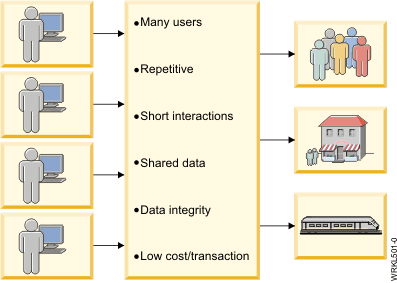
\includegraphics[width=25em]{figures/figure1.png}
\caption{Characteristics of Transactional Systems}
\label{fig:oltp}
\end{figure}
\par

Transaction systems must be able to support a high number of concurrent users and transaction types.
\par
One of the main characteristics of a transaction or online system is that the interactions between the user and the system are very brief. Most transactions are executed in short time periods--one second, in some cases. The user will perform a complete business transaction through short interactions, with immediate response time required for each interaction. These are mission-critical applications; therefore, continuous availability, high performance, and data protection and integrity are required.
\par
Online transaction processing (OLTP) is transaction processing that occurs interactively; it requires:
\begin{itemize}
\item Immediate response time
\item Continuous availability of the transaction interface to the end user
\item Security
\item Data integrity.
\end{itemize}
Online transactions are familiar to many people. Some examples include:
\begin{itemize}
\item ATM transactions such as deposits, withdrawals, inquiries, and transfers
\item Supermarket payments with debit or credit cards
\item Buying merchandise over the Internet.
\end{itemize}
\par
In fact, an online system has many of the characteristics of an operating system:
\begin{itemize}
\item Managing and dispatching tasks
\item Controlling user access authority to system resources
\item Managing the use of memory
\item Managing and controlling simultaneous access to data files
\item Providing device independence.
\end{itemize}
\par
Transactional systems are databases that record a company’s daily transactions. The three major transactional databases include CRM (customer relationship management), HRM (human resources management), and ERP (enterprise resource planning). For instance, a sales transaction would be recorded and stored as a piece of data in the CRM database.
\par
Transactional systems are not considered optimal for business intelligence. This is for a variety of reasons, including the fact that a) data is not optimized for reporting and analysis and b) querying directly against these databases may slow down the system and prevent the databases from recording transactions in real time.
\par
In some cases, companies use an ETL tool to collect data from their transactional databases, transform them to be optimized for BI, and load them into a data warehouse or other data mart. The main downside of this approach is that a data warehouse is a complex and expensive architecture, which is why many other companies opt to report directly against their transactional databases.
\par
A transaction process system and transaction processing are often contrasted with a batch process system and batch processing, where many requests are all executed at one time. The former requires the interaction of a user, whereas batch processing does not require user involvement. In batch processing the results of each transaction are not immediately available. Additionally, there is a delay while the many requests are being organized, stored and eventually executed. In transaction processing there is no delay and the results of each transaction are immediately available. During the delay time for batch processing, errors can occur. Although errors can occur in transaction processing, they are infrequent and tolerated, but do not warrant shutting down the entire system.
\par
To achieve performance, reliability and consistency, data must be readily accessible in a data warehouse, backup procedures must be in place and the recovery process must be in place to deal with system failure, human failure, computer viruses, software applications or natural disasters.
\par
\section{Objectives}
Objective of the system is to provide a better solution to manage college activities in an efficient manner and increase the productivity of the system.
\begin{enumerate}
\item To convert all offline process into online.
\item Improve service experience.
\item Less maintenance cost and time saving.
\item Development of Software Development Kit (SDKs) for future developments.
\item Designing of API based architecture to achieve maximum cross-compatibility.
\end{enumerate}
\section{Project Scope}
Expectations for improved performance are always increasing, higher education leaders continue to think more creatively about how their people, process and technology can work together more efficiently. The transactional system will support this view by helping institutions build, manage and extend their digital campus. It enables individuals, systems and communities to interact seamlessly across campus in an environment where efficiency, service delivery and personalized education experiences propel desired outcomes. This project aims to convert manual procedures into an automated single software.